\documentclass[a4paper,11pt]{jsarticle}
\usepackage{amsmath,amssymb} %AMS-LaTeX
\usepackage{epstopdf} % For handling bounding box issue
\usepackage[dvipdfmx]{graphicx} % For including graphics
\usepackage{float}

\begin{document}
\section{Prophet Modelの仕組み}
\subsection{モデルの概要}
\begin{frame}
  
時系列データは、トレンド + 季節要因 + ノイズ などの複数の要素から成り立っていて、これらの要素に分解することで理論値の予測ができる、という考え方があります。
    
Prophetでは、時系列は下記のような構成要素をもつと捉えています。

    \begin{itemize}
      \item g(t):トレンド関数
      \item s(t):季節性変化
      \item h(t):休日効果
      \item $ \epsilon $t:誤差項
    \end{itemize}

さらに、時系列はこれらの要素の和と捉え下記のようなモデル式を組み立てています。
\begin{equation*}
  y(t)=g(t)+s(t)+h(t)+\epsilon t
\end{equation*}

\section{ARIMAモデルの仕組み}
\subsection{ARIMAは自己回帰和分移動平均(AutoRegressive Integrated Moving Average)の略称}
自己回帰モデリングと移動平均モデリングは、時系列データを予測するための2つの異なるアプローチです。ARIMAはこれら2つのアプローチを統合しているため、この名前が付けられています。予測は、時系列の過去の動作を使用して、その時系列の1つ以上の将来の値を予測する機械学習の一分野です。小さな店でアイスクリームを買うことを想像してみてください。天候の温暖化に伴い、アイスクリームの売上が着実に増加していることをご存じであれば、おそらく来週の注文は、この数週間の注文よりも少し増えるはずだと予測できるでしょう。どの程度大きくなるかは、今週の売上が前週の売上とどれだけ異なるかによって決まります。比較する過去がなければ未来を予測することはできないため、過去の時系列データはARIMAばかりではなく、すべての予測手法や時系列分析手法にとって非常に重要です。

詳しくは、(https://shorturl.at/FZMuA)を参照してください。
\end{frame}  


  

\section{LSTMの紹介}
\subsection{LSTM(長・短期記憶)とは}
LSTMとは、AIが機械学習を行うための仕組みであるニューラルネットワークの一種です。LSTMは「Long Short Term Memory」の略称で、日本語では「長・短期記憶」と訳されます。
他のニューラルネットワークと同様に、LSTMは入力された情報をもとに、機械学習モデルを構築することが可能です。LSTMが開発される以前のニューラルネットワークでは、長い文章データなどの学習に課題がありました。従来のニューラルネットワークの弱点を補強し、長いデータでも高い精度で学習できるようになったことがLSTMの特長です。
\subsection{LSTMとRNNの違い}
LSTMは、RNNと呼ばれるニューラルネットワークを改良したものです。RNNは「Recurrent Neural Network」の略称で、日本語では「回帰型ニューラルネットワーク」と訳されます。RNNは、時間に伴って変化するデータを学習できることが特徴です。音声認識や株価の予測などにRNNが応用されています。

LSTMとRNNの違いは、記憶セルと呼ばれる仕組みの有無です。RNNには記憶セルが無く、ニューラルネットワークのある層で計算された情報がそのまま次の層へと引き継がれます。一方、LSTMには記憶セルがあり、入力された情報の一部を保ったまま機械学習を行うことが可能です。

記憶セルを持たないRNNでは、数多くの層で計算が行われる過程で「勾配」と呼ばれる特徴量が消失し、機械学習が進まなくなってしまう問題がありました。LSTMは記憶セルに必要なデータを残しながら計算を行うことで、勾配消失問題を解決しています。
\subsection{LSTMの仕組み}
\subsubsection{忘却ゲート}
忘却ゲートでは、入力された情報をもとに、記憶セルに保存されているデータをどれだけ忘れるかが決定されます。機械学習のプロセスにおいて、記憶セルのデータをすべて消去する必要がある場合、忘却ゲートから出力される数値は0です。一方、記憶セルのデータをすべて残しておく場合は1が出力されます。記憶セルのデータを忘れる度合いに応じて、0から1までの値を出力することが忘却ゲートの機能です。
\subsubsection{入力ゲート}
入力ゲートは、入力された情報の中から、新たに記憶セルに保存するべき情報を決定します。また、シグモイド関数と呼ばれる仕組みで、各入力の重要度を0から1の範囲の値で決めることも入力ゲートの役割です。入力ゲートで算出された値は記憶セルのデータと掛け合わされ、出力ゲートへと引き渡されます。
\subsubsection{出力ゲート}
出力ゲートの役割は、最終的に出力する情報の決定です。入力ゲートまでで処理された情報に対して、重要度に応じた重みづけを行い、出力するデータを計算します。

LSTMはこれらのプロセスを通じて保持すべきデータを取捨選択し、高い精度で機械学習を行うことが可能です。

LSTMはRNNを改良したニューラルネットワークです。入力情報の一部を記憶する仕組みにより、文章生成などの自然言語処理を実現できます。また、音声認識や株価予測など、さまざまな分野で活用されています。

\begin{figure}[H]  
  \centering  
  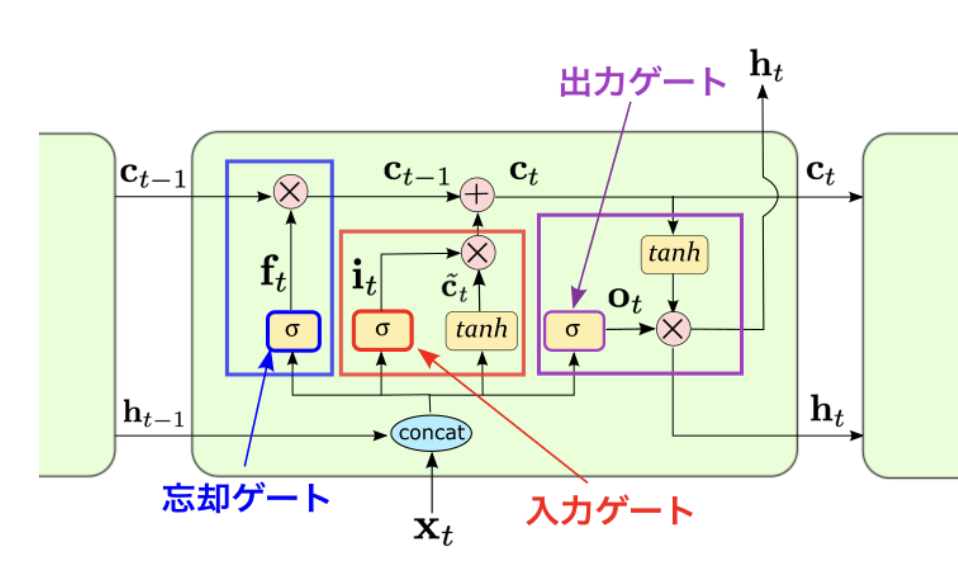
\includegraphics[width=0.6\textwidth]{pic/lstm1.png}  
  \caption{LSTMネットワークの構造}  
  \label{fig:lstm1}  
\end{figure}  
\vspace{1em}

\section{予測精度の評価指標}
予測精度の評価指標は、RMSE(二乗平均平方根誤差、Root Mean Squared Error)とMAE(平均絶対誤差、Mean Absolute Error)、MAPE(平均絶対パーセント誤差、Mean absolute percentage error)を使います。  

以下の記号を使い精度指標の説明をします。  

\begin{itemize}  
\item $y_i^{actual}$ \, ... \, $i$番目の実測値  
\item $y_i^{pred}$ \, ... \, $i$番目の予測値  
\item $n$ \, ... \, 実測値・予測値の数  
\end{itemize}  

\section*{二乗平均平方根誤差(RMSE、Root Mean Squared Error)}  
\begin{equation}  
\sqrt{\frac{1}{n}\sum_{i=1}^n(y_i^{actual} - y_i^{pred})^2}  
\end{equation}  

\section*{平均絶対誤差(MAE、Mean Absolute Error)}  
\begin{equation}  
\frac{1}{n}\sum_{i=1}^n|y_i^{actual} - y_i^{pred}|  
\end{equation}  

\section*{平均絶対パーセント誤差(MAPE、Mean absolute percentage error)}  
\begin{equation}  
\frac{1}{n}\sum_{i=1}^n|\frac{y_i^{actual} - y_i^{pred}}{y_i^{actual}}|  
\end{equation}  

\end{document}





